% ============================================================
% main.tex — Documento principal del proyecto SIRCA-RAG
% Formato: IEEE Conference Paper (doble columna, 6–10 páginas)
% Idioma: Español
% Estado: Investigación en progreso (fase teórica)
% ============================================================
\documentclass[conference]{IEEEtran}

% ============================================================
% PAQUETES ESENCIALES
% ============================================================

% --- Codificación y tipografía ---
\usepackage[utf8]{inputenc}
\usepackage[T1]{fontenc}
\usepackage[spanish,es-tabla]{babel}

% --- Matemáticas ---
\usepackage{amsmath,amssymb,amsfonts}
\usepackage{mathtools}

% --- Figuras y gráficos ---
\usepackage{graphicx}
\usepackage[font=small,labelfont=bf]{caption}
\usepackage{subcaption}
\graphicspath{{figures/}}

% --- Tablas profesionales ---
\usepackage{booktabs}
\usepackage{multirow}
\usepackage{array}
\usepackage{tabularx}

% --- Algoritmos ---
\usepackage[ruled,vlined,linesnumbered,spanish]{algorithm2e}

% --- Colores y enlaces ---
\usepackage[dvipsnames]{xcolor}
\usepackage[colorlinks=true,
            linkcolor=blue!70!black,
            citecolor=blue!70!black,
            urlcolor=blue!60!black]{hyperref}

% --- Código fuente ---
\usepackage{listings}
\lstset{
  basicstyle=\footnotesize\ttfamily,
  breaklines=true,
  frame=single,
  numbers=left,
  numberstyle=\tiny,
  keywordstyle=\color{blue},
  commentstyle=\color{gray},
  stringstyle=\color{red!70!black}
}

% --- Utilidades adicionales ---
\usepackage{enumitem}
\usepackage{balance}
\usepackage{url}
\usepackage{cite}
\usepackage{float}

% ============================================================
% COMANDOS PERSONALIZADOS
% ============================================================
% ============================================================
% custom_commands.tex
% Comandos personalizados para el proyecto SIRCA-RAG
% Facilita la consistencia terminológica y tipográfica
% ============================================================

% --- Nombre del sistema ---
\newcommand{\sirca}{\textsc{SIRCA-RAG}}
\newcommand{\sircafull}{Arquitectura Semi-Autónoma de Recuperación y Generación Contextual de Conocimiento Biomédico}

% --- Acrónimos frecuentes ---
\newcommand{\rag}{\textsc{RAG}}
\newcommand{\nlp}{\textsc{NLP}}
\newcommand{\llm}{\textsc{LLM}}
\newcommand{\llms}{\textsc{LLMs}}
\newcommand{\faiss}{\textsc{FAISS}}
\newcommand{\bert}{\textsc{BERT}}
\newcommand{\biobert}{\textsc{BioBERT}}
\newcommand{\scispacy}{\textsc{SciSpaCy}}
\newcommand{\mrr}{\textsc{MRR}}

% --- Operadores matemáticos ---
\DeclareMathOperator{\simcos}{sim_{cos}}
\DeclareMathOperator{\argmax}{arg\,max}
\DeclareMathOperator{\argmin}{arg\,min}
\DeclareMathOperator{\softmax}{softmax}
\DeclareMathOperator{\topk}{top\text{-}k}
\DeclareMathOperator{\embed}{Embed}
\DeclareMathOperator{\retrieve}{Retrieve}
\DeclareMathOperator{\rerank}{Rerank}
\DeclareMathOperator{\generate}{Generate}
\DeclareMathOperator{\ground}{Ground}
\DeclareMathOperator{\score}{score}

% --- Notación vectorial ---
\newcommand{\vect}[1]{\mathbf{#1}}
\newcommand{\query}{\vect{q}}
\newcommand{\doc}{\vect{d}}
\newcommand{\emb}[1]{\vect{e}_{#1}}

% --- Conjuntos y colecciones ---
\newcommand{\corpus}{\mathcal{C}}
\newcommand{\documents}{\mathcal{D}}
\newcommand{\knowledge}{\mathcal{K}}
\newcommand{\memory}{\mathcal{M}}
\newcommand{\sources}{\mathcal{S}}

% --- Funciones de scoring ---
\newcommand{\fsim}{f_{\text{sim}}}
\newcommand{\frel}{f_{\text{rel}}}
\newcommand{\fground}{f_{\text{ground}}}
\newcommand{\ffaith}{f_{\text{faith}}}

% --- Etiquetas de componentes ---
\newcommand{\componentone}{\textbf{C1}}
\newcommand{\componenttwo}{\textbf{C2}}
\newcommand{\componentthree}{\textbf{C3}}
\newcommand{\componentfour}{\textbf{C4}}
\newcommand{\componentfive}{\textbf{C5}}

% --- Formato de métricas ---
\newcommand{\metric}[1]{\texttt{#1}}
\newcommand{\recallk}{\metric{Recall@K}}
\newcommand{\precisionk}{\metric{Precision@K}}
\newcommand{\bertscore}{\metric{BERTScore}}

% --- Herramientas y tecnologías ---
\newcommand{\tool}[1]{\texttt{#1}}
\newcommand{\python}{\tool{Python}}
\newcommand{\fastapi}{\tool{FastAPI}}
\newcommand{\langchain}{\tool{LangChain}}
\newcommand{\llamaindex}{\tool{LlamaIndex}}
\newcommand{\chromadb}{\tool{ChromaDB}}

% --- Notas internas (ocultas en versión final) ---
\newcommand{\notainterna}[1]{} % Desactivar para versión final
% \newcommand{\notainterna}[1]{\textcolor{red}{\textbf{[NOTA:} #1\textbf{]}}}


% ============================================================
% METADATOS DEL DOCUMENTO
% ============================================================
\title{SIRCA-RAG: Arquitectura Semi-Autónoma de Recuperación y Generación Contextual de Conocimiento Biomédico mediante RAG Continuo, Memoria Vectorial y Adquisición Científica Automatizada aplicada a Plantas Medicinales Peruanas}

\author{
  \IEEEauthorblockN{Ower Frank Lopez Arela}
  \IEEEauthorblockA{Escuela Profesional de Ingeniería de Sistemas\\
    Universidad Nacional de San Agustín de Arequipa\\
    Arequipa, Perú\\
    olopeza@unsa.edu.pe}
  \and
  \IEEEauthorblockN{Daniel Enrique Marron Carcausto}
  \IEEEauthorblockA{Escuela Profesional de Ingeniería de Sistemas\\
    Universidad Nacional de San Agustín de Arequipa\\
    Arequipa, Perú\\
    dmarron@unsa.edu.pe}
}

% ============================================================
% INICIO DEL DOCUMENTO
% ============================================================
\begin{document}

\maketitle

% --- Abstract y palabras clave ---
% ============================================================
% abstract.tex — Resumen y palabras clave
% Estado: Investigación en progreso (enfoque teórico-conceptual)
% ============================================================

\begin{abstract}
La fragmentación del conocimiento biomédico sobre plantas medicinales peruanas constituye una barrera significativa para la investigación farmacológica y etnobotánica regional. La evidencia científica sobre compuestos bioactivos, propiedades terapéuticas y aplicaciones farmacológicas de especies como \textit{Uncaria tomentosa}, \textit{Lepidium meyenii} y \textit{Croton lechleri} se encuentra dispersa en múltiples repositorios, bases de datos biomédicas y literatura heterogénea, dificultando su recuperación contextualizada y sistematización. Los sistemas de búsqueda convencionales, basados en concordancia léxica, presentan limitaciones críticas en dominios especializados, mientras que los modelos generativos de lenguaje exhiben fenómenos de alucinación que comprometen la fiabilidad de las respuestas en contextos biomédicos.

El presente trabajo presenta los fundamentos teóricos y el diseño conceptual de \sirca{}, una arquitectura semi-autónoma de descubrimiento científico biomédico que integra: (i)~un pipeline de Retrieval-Augmented Generation especializado para literatura biomédica; (ii)~memoria vectorial persistente basada en embeddings semánticos; (iii)~un agente semi-autónomo con estrategias híbridas de retrieval y reranking contextual; (iv)~un sistema de adquisición científica automatizada; y (v)~generación contextualizada con grounding documental. Este artículo se centra en la fundamentación teórica de la propuesta, el análisis del estado del arte en sistemas RAG biomédicos y la definición arquitectónica conceptual del sistema, estableciendo las bases para su implementación y evaluación experimental en fases posteriores de la investigación.
\end{abstract}

\begin{IEEEkeywords}
Retrieval-Augmented Generation, memoria vectorial, NLP biomédico, plantas medicinales peruanas, recuperación semántica, grounding documental, embeddings biomédicos, etnobotánica computacional.
\end{IEEEkeywords}


% --- Secciones principales (desarrolladas) ---
% ============================================================
% introduction.tex — Sección I: Introducción
% Integra: contexto, problemática, motivación, contribuciones
% ============================================================

\section{Introducción}
\label{sec:introduction}

El descubrimiento de conocimiento biomédico a partir de fuentes científicas heterogéneas constituye uno de los desafíos fundamentales de la inteligencia artificial aplicada a ciencias de la salud~\cite{lee2020biobert, gu2021domain}. En particular, la investigación sobre plantas medicinales en regiones de alta biodiversidad, como Perú, enfrenta barreras estructurales derivadas de la fragmentación documental, la dispersión de evidencia farmacológica y la ausencia de infraestructuras computacionales especializadas capaces de sistematizar, recuperar y contextualizar el conocimiento científico disponible~\cite{heinrich2020ethnopharmacology}.

Perú alberga aproximadamente 25\,000 especies vegetales, de las cuales se estima que entre 1\,400 y 5\,000 poseen propiedades medicinales documentadas en sistemas de conocimiento tradicional~\cite{bussmann2015toxicity}. Especies como \textit{Uncaria tomentosa} (uña de gato), \textit{Lepidium meyenii} (maca), \textit{Croton lechleri} (sangre de grado) y \textit{Minthostachys mollis} (muña) han sido objeto de investigación farmacológica significativa, con evidencia sobre actividad antiinflamatoria, antioxidante, inmunomoduladora y citotóxica~\cite{lock2016uncaria, gonzales2012ethnobiology}. Sin embargo, esta evidencia permanece dispersa en artículos científicos, repositorios institucionales, bases de datos biomédicas y documentación técnica, dificultando su integración sistemática en procesos de investigación.

Los motores de búsqueda científicos convencionales operan predominantemente mediante concordancia léxica o modelos de relevancia superficial, presentando limitaciones significativas en dominios biomédicos especializados~\cite{wang2018clinical}: (i)~recuperación sin comprensión semántica profunda; (ii)~ausencia de contextualización disciplinar; (iii)~incapacidad de mantener memoria contextual entre sesiones; (iv)~falta de actualización continua del corpus; y (v)~desconexión entre recuperación y generación contextualizada~\cite{karpukhin2020dense}.

Paralelamente, los modelos generativos de lenguaje de gran escala (\llms{}) han demostrado capacidades notables en comprensión lingüística~\cite{brown2020language, touvron2023llama}, pero su aplicación directa en dominios biomédicos presenta riesgos sustanciales, particularmente el fenómeno de \textit{alucinación} —la generación de información factualmente incorrecta pero lingüísticamente coherente— que compromete la fiabilidad científica~\cite{ji2023survey}. El paradigma de Retrieval-Augmented Generation (\rag{}) ha emergido como estrategia para mitigar estas limitaciones~\cite{lewis2020retrieval, guu2020realm}, pero las implementaciones convencionales presentan restricciones en dominios especializados: dependencia de corpus estáticos, ausencia de adquisición continua y carencia de memoria vectorial persistente~\cite{siriwardhana2023improving}.

Frente a estas limitaciones, el presente trabajo propone \sirca{}, una arquitectura semi-autónoma de descubrimiento científico biomédico que integra cinco capacidades fundamentales: un pipeline \rag{} biomédico (\componentone{}), memoria vectorial persistente (\componenttwo{}), un agente semi-autónomo con retrieval híbrido (\componentthree{}), adquisición científica automatizada (\componentfour{}), y generación contextualizada con grounding documental (\componentfive{}).

\subsection{Contribuciones del trabajo}
\label{subsec:contributions}

Este artículo presenta las siguientes contribuciones:

\begin{enumerate}[label=(\roman*)]
  \item El diseño conceptual de una arquitectura semi-autónoma de descubrimiento científico biomédico que integra adquisición continua de literatura, retrieval contextual, memoria vectorial persistente y generación contextualizada, orientada al dominio de plantas medicinales peruanas.

  \item La formulación teórica de un pipeline \rag{} especializado que combina retrieval híbrido, reranking contextual biomédico y grounding documental para la reducción de alucinaciones.

  \item Un análisis comprehensivo del estado del arte en sistemas \rag{}, NLP biomédico, bases de datos vectoriales y recuperación semántica, contextualizando las oportunidades y limitaciones para el dominio etnobotánico.

  \item La definición de un marco de evaluación experimental para fases posteriores de la investigación, identificando métricas y baselines apropiados para el dominio.
\end{enumerate}

\subsection{Organización del artículo}
\label{subsec:organization}

El artículo se organiza de la siguiente manera. La Sección~\ref{sec:related_work} analiza el estado del arte en sistemas \rag{} biomédicos y recuperación semántica. La Sección~\ref{sec:theoretical_framework} establece los fundamentos teóricos que sustentan la propuesta. La Sección~\ref{sec:architecture} presenta el diseño conceptual de la arquitectura de \sirca{}. La Sección~\ref{sec:methodology} describe la metodología y el plan de evaluación propuesto. La Sección~\ref{sec:experiments} define el marco de evaluación experimental planificado. Finalmente, la Sección~\ref{sec:conclusion} presenta las conclusiones preliminares y las líneas de trabajo futuro.

% ============================================================
% related_work.tex — Sección II: Trabajos Relacionados
% Estado: Desarrollado completamente
% ============================================================

\section{Trabajos Relacionados}
\label{sec:related_work}

Esta sección analiza las líneas de investigación relacionadas con la propuesta, organizadas en cuatro ejes temáticos fundamentales.

\subsection{Retrieval-Augmented Generation (RAG)}
\label{subsec:rw_rag}

El paradigma \rag{} fue formalizado por Lewis et al.~\cite{lewis2020retrieval}, quienes propusieron la combinación de un retriever con un generator para tareas de NLP intensivas en conocimiento, demostrando mejoras en factualidad y relevancia frente a modelos puramente paramétricos. Guu et al.~\cite{guu2020realm} introdujeron REALM, integrando la recuperación directamente en el pre-entrenamiento del modelo de lenguaje. Borgeaud et al.~\cite{borgeaud2022improving} escalaron la idea mediante RETRO, demostrando que modelos con acceso a bases de conocimiento externas de trillones de tokens alcanzan rendimiento competitivo con modelos significativamente más grandes.

Izacard y Grave~\cite{izacard2021leveraging} propusieron Fusion-in-Decoder, concatenando múltiples pasajes recuperados en el decoder. Asai et al.~\cite{asai2024selfrag} introdujeron Self-RAG, un framework que enseña al modelo a recuperar, generar y criticar sus propias respuestas mediante tokens de reflexión. Khattab y Zaharia~\cite{khattab2020colbert} desarrollaron ColBERT, un modelo de interacción tardía para búsquedas eficientes mediante representaciones contextualizadas. Gao et al.~\cite{gao2024retrieval} proporcionaron un survey comprehensivo del paradigma \rag{}, categorizando las aproximaciones según sus componentes de recuperación, aumentación y generación.

A pesar de estos avances, la aplicación de \rag{} en dominios biomédicos especializados permanece subexplorada. La mayoría de los sistemas operan sobre corpora genéricos y no incorporan mecanismos de adquisición continua ni memoria persistente.

\subsection{NLP biomédico y recuperación semántica}
\label{subsec:rw_bionlp}

Lee et al.~\cite{lee2020biobert} desarrollaron \biobert{}, un modelo basado en BERT pre-entrenado con artículos de PubMed y PMC, demostrando mejoras sustanciales en tareas de extracción biomédica y question answering. Gu et al.~\cite{gu2021domain} propusieron PubMedBERT, argumentando que el pre-entrenamiento desde cero con vocabulario especializado supera al pre-entrenamiento continuo. Neumann et al.~\cite{neumann2019scispacy} presentaron \scispacy{}, una extensión de spaCy optimizada para texto biomédico con modelos para NER y vinculación a ontologías como UMLS.

Luo et al.~\cite{luo2022biogpt} introdujeron BioGPT, un modelo generativo pre-entrenado para el dominio biomédico. Jin et al.~\cite{jin2019pubmedqa} crearon PubMedQA, un benchmark de referencia para question answering biomédico. Xiong et al.~\cite{xiong2021approximate} propusieron ANCE para mejorar la calidad de recuperación densa en dominios especializados. Nentidis et al.~\cite{nentidis2023overview} reportaron los avances del desafío BioASQ, evidenciando los retos persistentes en QA biomédico.

\subsection{Bases de datos vectoriales y memoria persistente}
\label{subsec:rw_vectordb}

Johnson et al.~\cite{johnson2021billion} desarrollaron \faiss{}, estableciendo los fundamentos algorítmicos (IVF, PQ, HNSW) para la búsqueda eficiente de vecinos más cercanos a escala. Reimers y Gurevych~\cite{reimers2019sentence} introdujeron Sentence-BERT, ampliamente adoptado para la representación vectorial de documentos. Sistemas como \chromadb{}, Milvus y Weaviate han democratizado el acceso a bases de datos vectoriales con persistencia nativa.

Park et al.~\cite{park2023generative} exploraron la integración de memoria a largo plazo en agentes generativos, donde las representaciones vectoriales de interacciones pasadas se almacenan para mantener coherencia contextual entre sesiones, una capacidad fundamental para la arquitectura propuesta en este trabajo.

\subsection{Sistemas para etnobotánica y farmacognosia}
\label{subsec:rw_ethnobotany}

Bussmann y Sharon~\cite{bussmann2006traditional} documentaron la flora medicinal del norte de Perú, proporcionando una base de datos de referencia. Heinrich et al.~\cite{heinrich2020ethnopharmacology} revisaron las aproximaciones computacionales a la etnofarmacología, identificando oportunidades para la aplicación de técnicas de IA. Gonzales~\cite{gonzales2012ethnobiology} proporcionó una revisión comprehensiva de la evidencia sobre \textit{Lepidium meyenii}. Chandak et al.~\cite{chandak2023building} exploraron grafos de conocimiento biomédico para la representación de relaciones entre compuestos y actividades biológicas.

\subsection{Posicionamiento de la propuesta}
\label{subsec:rw_positioning}

La Tabla~\ref{tab:related_work_comparison} resume el posicionamiento de \sirca{} frente a los sistemas revisados. Ningún sistema existente integra simultáneamente las cinco capacidades propuestas: pipeline \rag{} biomédico, memoria vectorial persistente, retrieval híbrido, adquisición continua y grounding documental, específicamente orientado al dominio etnobotánico.

% ============================================================
% related_work_table.tex — Tabla comparativa de trabajos relacionados
% ============================================================

\begin{table*}[!t]
\centering
\caption{Análisis comparativo de sistemas relacionados frente a las capacidades de \sirca{}.}
\label{tab:related_work_comparison}
\renewcommand{\arraystretch}{1.2}
\footnotesize
\begin{tabularx}{\textwidth}{l c c c c c c}
\toprule
\textbf{Sistema / Enfoque} & \textbf{RAG} & \textbf{Memoria} & \textbf{Retrieval} & \textbf{Adquisición} & \textbf{Grounding} & \textbf{Dominio} \\
 & \textbf{Biomédico} & \textbf{Persistente} & \textbf{Híbrido} & \textbf{Continua} & \textbf{Documental} & \textbf{Específico} \\
\midrule
RAG~\cite{lewis2020retrieval}                   & --          & --          & --          & --          & Parcial     & General \\
REALM~\cite{guu2020realm}                       & --          & --          & Denso       & --          & --          & General \\
Self-RAG~\cite{asai2024selfrag}                 & --          & --          & Denso       & --          & \checkmark  & General \\
ColBERT~\cite{khattab2020colbert}               & --          & --          & Denso       & --          & --          & General \\
BioBERT~\cite{lee2020biobert}                   & --          & --          & --          & --          & --          & Biomédico \\
BioGPT~\cite{luo2022biogpt}                     & --          & --          & --          & --          & --          & Biomédico \\
PubMedQA~\cite{jin2019pubmedqa}                 & --          & --          & --          & --          & Parcial     & Biomédico \\
S2ORC~\cite{lo2020s2orc}                        & --          & --          & --          & \checkmark  & --          & General \\
\midrule
\textbf{\sirca{} (propuesto)} & \checkmark  & \checkmark  & \checkmark  & \checkmark  & \checkmark  & \textbf{Etnobotánico} \\
\bottomrule
\end{tabularx}
\end{table*}


% ============================================================
% theoretical_framework.tex — Sección III: Marco Teórico
% Estado: COMPLETAMENTE DESARROLLADO (foco principal del paper)
% ============================================================

\section{Marco Teórico}
\label{sec:theoretical_framework}

Esta sección establece los fundamentos teóricos que sustentan la arquitectura propuesta, abarcando el paradigma de Retrieval-Augmented Generation, la representación vectorial semántica y modelos de embedding biomédicos, las bases de datos vectoriales y algoritmos de búsqueda aproximada, el procesamiento de lenguaje natural biomédico, las estrategias de retrieval híbrido y reranking contextual, los mecanismos de grounding documental, la memoria vectorial persistente y los sistemas multiagente para descubrimiento científico.

\subsection{Retrieval-Augmented Generation}
\label{subsec:tf_rag}

El paradigma de Retrieval-Augmented Generation constituye una extensión del framework generativo convencional mediante la incorporación de evidencia documental externa en el proceso de generación~\cite{lewis2020retrieval}. Formalmente, dado un modelo generativo $G_\theta$ parametrizado por $\theta$ y un componente de recuperación $R_\phi$ parametrizado por $\phi$, el sistema \rag{} genera una respuesta $y$ para una consulta $q$ como:

\begin{equation}
\label{eq:rag_general}
  P(y \mid q) = \sum_{d \in \topk(R_\phi(q, \corpus))} P_G(y \mid q, d) \cdot P_R(d \mid q)
\end{equation}

\noindent donde $\topk(R_\phi(q, \corpus))$ denota los $K$ documentos más relevantes recuperados del corpus $\corpus$ para la consulta $q$, $P_R(d \mid q)$ es la probabilidad de relevancia del documento $d$ y $P_G(y \mid q, d)$ es la probabilidad de generar $y$ condicionada en $q$ y $d$.

Lewis et al.~\cite{lewis2020retrieval} propusieron dos variantes. En RAG-Sequence, un único documento condiciona la generación de toda la secuencia de salida:

\begin{equation}
\label{eq:rag_sequence}
  P_{\text{RAG-Seq}}(y \mid q) = \sum_{d \in \topk} P_R(d \mid q) \prod_{i=1}^{n} P_G(y_i \mid q, d, y_{1:i-1})
\end{equation}

En RAG-Token, diferentes documentos pueden condicionar la generación de diferentes tokens, proporcionando mayor flexibilidad:

\begin{equation}
\label{eq:rag_token}
  P_{\text{RAG-Tok}}(y \mid q) = \prod_{i=1}^{n} \sum_{d \in \topk} P_R(d \mid q) \cdot P_G(y_i \mid q, d, y_{1:i-1})
\end{equation}

La ventaja fundamental de \rag{} sobre modelos puramente paramétricos reside en la separación entre el conocimiento almacenado en los parámetros del modelo y el conocimiento accesible mediante recuperación, permitiendo la actualización del conocimiento sin re-entrenamiento. Gao et al.~\cite{gao2024retrieval} categorizaron las arquitecturas \rag{} contemporáneas en tres paradigmas: \textit{Naive RAG}, que implementa la cadena indexación-recuperación-generación; \textit{Advanced RAG}, que incorpora optimizaciones pre y post-retrieval; y \textit{Modular RAG}, que descompone el pipeline en módulos reconfigurables. La arquitectura propuesta en este trabajo se alinea con el paradigma Modular RAG, extendido con capacidades de adquisición continua y memoria persistente.

\subsubsection{RAG en dominios especializados}

La aplicación de \rag{} en dominios especializados introduce desafíos adicionales que los sistemas genéricos no abordan~\cite{siriwardhana2023improving}. En el dominio biomédico, la terminología especializada, las relaciones semánticas complejas entre entidades (compuestos, especies, actividades biológicas) y la necesidad de trazabilidad bibliográfica imponen requisitos específicos sobre los componentes de recuperación y generación. Los modelos de embedding genéricos frecuentemente fallan en capturar relaciones disciplinares, como la asociación entre ``alcaloide oxindólico'' y ``oxindole alkaloid'', o entre nombres taxonómicos y nombres comunes de especies medicinales.

\subsection{Embeddings semánticos y representación vectorial}
\label{subsec:tf_embeddings}

Los embeddings semánticos proporcionan representaciones numéricas de alta dimensionalidad que capturan relaciones semánticas entre textos~\cite{reimers2019sentence}. Formalmente, una función de embedding $\embed: \mathcal{T} \rightarrow \mathbb{R}^d$ proyecta un texto $t \in \mathcal{T}$ a un vector en un espacio $d$-dimensional, donde la proximidad geométrica refleja similitud semántica.

La similitud entre dos textos $t_1$ y $t_2$ se cuantifica mediante la similitud coseno:

\begin{equation}
\label{eq:cosine_similarity}
  \simcos(\emb{t_1}, \emb{t_2}) = \frac{\emb{t_1} \cdot \emb{t_2}}{\|\emb{t_1}\| \cdot \|\emb{t_2}\|}
\end{equation}

\noindent donde $\emb{t_i} = \embed(t_i) \in \mathbb{R}^d$ denota la representación vectorial del texto $t_i$.

\subsubsection{Sentence Transformers y redes siamesas}

El framework Sentence-BERT~\cite{reimers2019sentence} extiende los modelos BERT mediante redes siamesas para producir embeddings de oraciones semánticamente ricos. La arquitectura emplea una estructura siamesa donde dos instancias del mismo modelo procesan pares de oraciones, y una función de pooling genera las representaciones finales:

\begin{equation}
\label{eq:sbert}
  \emb{s} = \text{MeanPool}(\text{BERT}(s)) \in \mathbb{R}^d
\end{equation}

El entrenamiento se realiza optimizando la pérdida de tripleta:

\begin{equation}
\label{eq:triplet_loss}
  \mathcal{L} = \max\left(0, \|\emb{a} - \emb{p}\| - \|\emb{a} - \emb{n}\| + \epsilon\right)
\end{equation}

\noindent donde $\emb{a}$, $\emb{p}$ y $\emb{n}$ representan los embeddings del anchor, positivo y negativo, y $\epsilon$ es el margen de separación. Esta formulación asegura que textos semánticamente similares se proyecten a regiones próximas del espacio vectorial.

\subsubsection{Embeddings biomédicos especializados}

En el dominio biomédico, los modelos de embedding genéricos presentan limitaciones para capturar relaciones terminológicas específicas. \biobert{}~\cite{lee2020biobert}, pre-entrenado con 4.5 mil millones de palabras de PubMed y 13.5 mil millones de PMC, produce representaciones que capturan relaciones disciplinares con mayor fidelidad. PubMedBERT~\cite{gu2021domain}, pre-entrenado desde cero con vocabulario exclusivamente biomédico, demostró que la construcción de vocabulario in-domain supera consistentemente al pre-entrenamiento continuo en benchmarks como BLURB (\textit{Biomedical Language Understanding and Reasoning Benchmark}).

Para el dominio de plantas medicinales peruanas, la selección del modelo de embedding es crítica. Términos como \textit{Uncaria tomentosa}, ``mitrafilina'', ``actividad inmunomoduladora'' y ``alcaloide pentacíclico'' requieren representaciones que capturen correctamente su proximidad semántica a pesar de la variabilidad léxica y multilingüe inherente a la literatura etnobotánica.

\subsection{Bases de datos vectoriales y búsqueda aproximada}
\label{subsec:tf_vectordb}

La búsqueda eficiente de documentos semánticamente relevantes requiere algoritmos de \textit{Approximate Nearest Neighbor} (ANN) que ofrezcan un balance entre precisión y eficiencia computacional. \faiss{}~\cite{johnson2021billion} implementa múltiples estrategias:

\begin{itemize}[leftmargin=*]
  \item \textbf{Inverted File Index (IVF):} Particiona el espacio vectorial en $n_{\text{list}}$ celdas de Voronoi, restringiendo la búsqueda a las $n_{\text{probe}}$ celdas más cercanas al vector de consulta. La complejidad se reduce de $O(N \cdot d)$ a $O(n_{\text{probe}} \cdot N/n_{\text{list}} \cdot d)$.

  \item \textbf{Product Quantization (PQ):} Comprime vectores de alta dimensionalidad mediante cuantización del espacio en subespacios, reduciendo requisitos de memoria y acelerando el cálculo de distancias.

  \item \textbf{Hierarchical Navigable Small World (HNSW):} Construye un grafo multicapa navegable que permite búsqueda eficiente con complejidad logarítmica $O(\log N)$, ofreciendo alta recall con latencia predecible.
\end{itemize}

Sistemas como \chromadb{}, Milvus y Weaviate extienden estas capacidades con persistencia nativa, filtrado por metadatos y APIs simplificadas, democratizando la construcción de sistemas de memoria vectorial. Para un corpus biomédico de escala moderada ($N < 10^6$ documentos), los índices IVF-Flat o HNSW proporcionan un balance adecuado entre precisión y rendimiento con recursos computacionales accesibles.

\subsection{NLP biomédico}
\label{subsec:tf_bionlp}

El procesamiento de lenguaje natural biomédico abarca técnicas especializadas para el análisis computacional de textos científicos en ciencias de la salud~\cite{lee2020biobert}. Los componentes fundamentales para la arquitectura propuesta incluyen:

\subsubsection{Reconocimiento de entidades biomédicas (BioNER)}

La identificación automática de entidades biomédicas en texto no estructurado constituye una tarea fundamental. \scispacy{}~\cite{neumann2019scispacy} proporciona pipelines de NER pre-entrenados con capacidad de vinculación a ontologías como UMLS (\textit{Unified Medical Language System}), MeSH (\textit{Medical Subject Headings}) y ChEBI (\textit{Chemical Entities of Biological Interest}).

En el contexto de plantas medicinales peruanas, el BioNER debe identificar cuatro categorías de entidades: (a)~nombres taxonómicos (\textit{Uncaria tomentosa}, \textit{Lepidium meyenii}); (b)~compuestos químicos (mitrafilina, isomitrafilina, macamidas, taspina); (c)~actividades biológicas (actividad citotóxica, antiinflamatoria, antioxidante); y (d)~nombres vernáculos (uña de gato, maca, sangre de grado).

\subsubsection{Extracción de relaciones biomédicas}

La extracción de relaciones entre entidades permite construir representaciones estructuradas del conocimiento. Las relaciones relevantes incluyen:
\begin{itemize}[leftmargin=*]
  \item \texttt{PLANTA -- contiene -- COMPUESTO}
  \item \texttt{COMPUESTO -- exhibe -- ACTIVIDAD\_BIOLÓGICA}
  \item \texttt{PLANTA -- se\_usa\_para -- CONDICIÓN\_MÉDICA}
  \item \texttt{ESTUDIO -- reporta -- EFECTO\_FARMACOLÓGICO}
\end{itemize}

Estas relaciones, extraídas automáticamente mediante modelos de relación biomédica, enriquecen los metadatos del corpus y permiten filtrado semántico durante la recuperación.

\subsubsection{Segmentación semántica de documentos}

La segmentación de documentos en chunks semánticos constituye una etapa crítica del pipeline \rag{}. Dado un documento $d$ de longitud $L$ tokens, la segmentación produce una secuencia $\{c_1, c_2, \ldots, c_n\}$ donde:

\begin{equation}
\label{eq:chunking}
  c_i = d[i \cdot (w - o) : i \cdot (w - o) + w], \quad |c_i| = w, \quad o < w
\end{equation}

\noindent con tamaño de ventana $w$ y solapamiento $o$. La preservación de fronteras de oración y párrafo durante la segmentación es fundamental para mantener la coherencia semántica de cada fragmento, particularmente en textos biomédicos donde la ruptura de una descripción farmacológica puede alterar su significado.

\subsection{Retrieval híbrido}
\label{subsec:tf_hybrid_retrieval}

El retrieval híbrido combina métodos de recuperación dispersa (\textit{sparse}) y densa (\textit{dense}) para aprovechar las fortalezas complementarias de ambos paradigmas~\cite{karpukhin2020dense}. Formalmente, la puntuación híbrida de un documento $d$ para una consulta $q$ se define como:

\begin{equation}
\label{eq:hybrid_retrieval}
  \score_{\text{híb}}(q, d) = \alpha \cdot \score_{\text{denso}}(q, d) + (1 - \alpha) \cdot \score_{\text{disperso}}(q, d)
\end{equation}

\noindent donde $\alpha \in [0, 1]$ controla la ponderación relativa. El componente disperso se calcula típicamente mediante BM25:

\begin{equation}
\label{eq:bm25}
  \text{BM25}(q, d) = \sum_{t \in q} \text{IDF}(t) \cdot \frac{f(t, d) \cdot (k_1 + 1)}{f(t, d) + k_1 \cdot \left(1 - b + b \cdot \frac{|d|}{d_{\text{avg}}}\right)}
\end{equation}

\noindent donde $f(t, d)$ es la frecuencia del término $t$ en $d$, $|d|$ es la longitud del documento, $d_{\text{avg}}$ es la longitud promedio en el corpus, y $k_1$, $b$ son hiperparámetros de regularización.

La combinación híbrida es particularmente beneficiosa en dominios biomédicos, donde las consultas contienen tanto términos técnicos específicos —mejor capturados por métodos dispersos— como conceptos semánticos complejos —mejor capturados por métodos densos. Por ejemplo, una consulta sobre ``alcaloides oxindólicos de \textit{Uncaria tomentosa} con actividad antiinflamatoria'' combina términos químicos específicos con relaciones farmacológicas que requieren comprensión semántica.

\subsection{Reranking contextual}
\label{subsec:tf_reranking}

El reranking contextual constituye una etapa de refinamiento posterior a la recuperación inicial~\cite{nogueira2019passage}. Mientras los modelos bi-encoder utilizados en la recuperación inicial generan representaciones independientes para la consulta y el documento, los cross-encoders procesan simultáneamente ambos textos:

\begin{equation}
\label{eq:reranking}
  \score_{\text{rerank}}(q, d) = \sigma\left(\vect{w}^\top \cdot f_{\text{cross}}([q; \text{SEP}; d]) + b\right)
\end{equation}

\noindent donde $f_{\text{cross}}$ denota la representación producida por un modelo cross-encoder que procesa la concatenación de la consulta y el documento, $\sigma$ es la función sigmoide, y $\vect{w}$, $b$ son parámetros aprendidos. Esta arquitectura captura interacciones semánticas profundas entre la consulta y cada documento a costa de mayor complejidad computacional, por lo cual se aplica exclusivamente sobre los $K$ candidatos recuperados en la etapa anterior, seleccionando los $K' < K$ más relevantes.

\subsection{Grounding documental}
\label{subsec:tf_grounding}

El grounding documental es el proceso mediante el cual las respuestas generadas se fundamentan explícitamente en evidencia documental recuperada, reduciendo el riesgo de alucinaciones~\cite{ji2023survey}. Formalmente, una respuesta $r$ se considera \textit{grounded} respecto a un conjunto de documentos $\documents_k = \{d_1, \ldots, d_k\}$ si:

\begin{equation}
\label{eq:grounding}
  \fground(r, \documents_k) = \frac{|\{s_i \in r : \exists\, d_j \in \documents_k, \text{soporta}(d_j, s_i)\}|}{|\{s_i \in r\}|}
\end{equation}

\noindent donde $s_i$ denota las afirmaciones factuales en $r$ y $\text{soporta}(d_j, s_i)$ indica que $s_i$ puede ser verificada mediante $d_j$. Un valor alto de $\fground$ indica que la respuesta está bien fundamentada en la evidencia recuperada.

En dominios biomédicos, el grounding es particularmente crítico. Una afirmación sobre la actividad antiinflamatoria de un compuesto vegetal debe estar respaldada por estudios específicos, no por generalización del modelo. La implementación del grounding involucra: (i)~inclusión explícita de fragmentos documentales en el prompt; (ii)~instrucciones que requieren citación de fuentes; y (iii)~verificación posterior de consistencia.

\subsection{Memoria vectorial persistente}
\label{subsec:tf_memory}

La memoria vectorial persistente extiende las bases de datos vectoriales con capacidades de acumulación temporal y gestión de contexto entre sesiones. Formalmente, la memoria $\memory$ se define como:

\begin{equation}
\label{eq:memory}
  \memory = \{(\emb{d_i}, m_i, \tau_i) : d_i \in \corpus\}
\end{equation}

\noindent donde $\emb{d_i} \in \mathbb{R}^d$ es la representación vectorial, $m_i$ denota los metadatos (fuente, fecha, autores, tipo de documento) y $\tau_i$ es la marca temporal de incorporación.

Las operaciones fundamentales sobre $\memory$ incluyen:
\begin{itemize}[leftmargin=*]
  \item \textbf{Inserción:} $\memory \leftarrow \memory \cup \{(\embed(d), m, \tau_{\text{now}})\}$
  \item \textbf{Consulta semántica:} $\retrieve(\query, \memory, K) = \topk_{(\emb{d}, m, \tau) \in \memory} \simcos(\query, \emb{d})$
  \item \textbf{Consulta filtrada:} $\retrieve(\query, \memory, K, \mathcal{F}) = \topk_{(\emb{d}, m, \tau) \in \memory, \mathcal{F}(m)} \simcos(\query, \emb{d})$
  \item \textbf{Actualización incremental:} $\memory_{t+1} = \memory_t \cup \embed(\Delta\corpus_t)$
\end{itemize}

\noindent donde $\mathcal{F}$ es un predicado de filtrado sobre metadatos y $\Delta\corpus_t$ denota los documentos adquiridos en el período $t$. Esta capacidad de actualización incremental es fundamental para la adquisición científica continua propuesta en \sirca{}.

\subsection{Sistemas multiagente para descubrimiento científico}
\label{subsec:tf_multiagent}

Los sistemas multiagente proporcionan un paradigma organizacional donde agentes especializados colaboran para resolver tareas complejas~\cite{wooldridge2009introduction}. En el contexto de descubrimiento científico biomédico, la arquitectura multiagente permite la descomposición funcional del proceso en roles especializados:

\begin{itemize}[leftmargin=*]
  \item \textbf{Agente de adquisición:} Identificación, descarga y preprocesamiento de nueva literatura biomédica desde APIs científicas (PubMed, CrossRef, Semantic Scholar).
  \item \textbf{Agente de indexación:} Generación de embeddings, segmentación semántica y actualización de la memoria vectorial.
  \item \textbf{Agente de retrieval:} Ejecución de estrategias de recuperación híbrida y reranking contextual.
  \item \textbf{Agente de generación:} Producción de respuestas contextualizadas con grounding documental y citaciones.
  \item \textbf{Agente de verificación:} Validación de consistencia factual y fundamentación bibliográfica.
\end{itemize}

La coordinación entre agentes se propone mediante un orquestador central que selecciona dinámicamente las estrategias de procesamiento en función del tipo de consulta, el estado de la memoria vectorial y la disponibilidad de evidencia documental. Esta descomposición modular facilita la extensibilidad del sistema y permite la adición de nuevas capacidades sin reestructuración de los componentes existentes.


% --- Secciones en desarrollo (conceptuales) ---
% ============================================================
% architecture.tex — Sección IV: Arquitectura Propuesta
% Estado: Diseño conceptual (sin implementación)
% ============================================================

\section{Arquitectura Propuesta de SIRCA-RAG}
\label{sec:architecture}

Esta sección presenta el diseño conceptual de la arquitectura de \sirca{}, describiendo sus cinco componentes fundamentales y sus interacciones. La Figura~\ref{fig:architecture} ilustra la visión general del sistema propuesto.

\begin{figure}[!t]
  \centering
  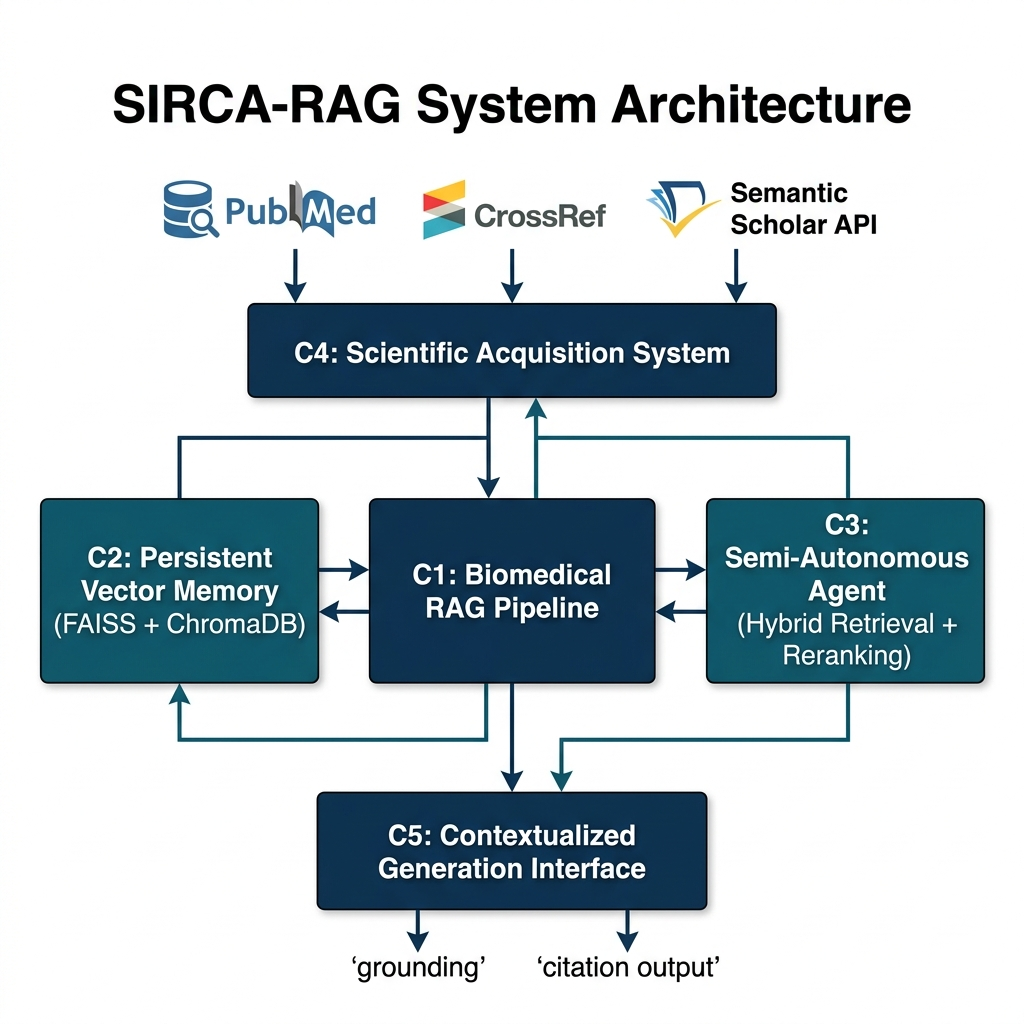
\includegraphics[width=\columnwidth]{sirca_architecture.png}
  \caption{Arquitectura conceptual de \sirca{}. El sistema integra cinco componentes: pipeline RAG biomédico (C1), memoria vectorial persistente (C2), agente semi-autónomo (C3), adquisición científica automatizada (C4) e interfaz de generación contextualizada (C5).}
  \label{fig:architecture}
\end{figure}

\subsection{Componentes del sistema}
\label{subsec:arch_components}

La arquitectura se articula en cinco componentes fundamentales diseñados para abordar las limitaciones identificadas en la Sección~\ref{sec:introduction}:

\textbf{C1 — Pipeline RAG biomédico:} Constituye el componente central de procesamiento. Su función es transformar documentos biomédicos heterogéneos (PDFs, XML de PubMed, HTML) en representaciones semánticas consultables, articulando el flujo completo de ingesta, segmentación, vectorización, recuperación y generación contextualizada.

\textbf{C2 — Memoria vectorial persistente:} Implementa un sistema de almacenamiento semántico que mantiene representaciones vectoriales, metadatos estructurados y relaciones documentales entre sesiones. Se propone una arquitectura de tres capas: capa vectorial (\faiss{}/\chromadb{}), capa de metadatos (PostgreSQL) y capa de sesión (Redis).

\textbf{C3 — Agente semi-autónomo:} Implementa la lógica de decisión del sistema, clasificando consultas (factuales, exploratorias, comparativas) y seleccionando dinámicamente la estrategia de retrieval, el nivel de reranking y las fuentes a consultar.

\textbf{C4 — Adquisición científica automatizada:} Automatiza la incorporación continua de nueva literatura mediante conexión programática a APIs de PubMed, CrossRef, Semantic Scholar y Europe PMC, con deduplicación semántica e indexación incremental.

\textbf{C5 — Interfaz de generación contextualizada:} Produce respuestas biomédicas fundamentadas en evidencia documental, con citaciones explícitas, instrucciones de grounding y restricciones de dominio.

\subsection{Flujo de datos propuesto}
\label{subsec:arch_flow}

El flujo de datos principal sigue la secuencia: (1)~el usuario formula una consulta biomédica; (2)~el agente (C3) clasifica la consulta y selecciona la estrategia; (3)~el pipeline (C1) ejecuta retrieval híbrido y reranking sobre la memoria (C2); (4)~los documentos relevantes se incorporan al contexto de generación; (5)~el modelo produce una respuesta con citas; y (6)~paralelamente, el sistema de adquisición (C4) enriquece continuamente la memoria vectorial.

\subsection{Stack tecnológico propuesto}
\label{subsec:arch_stack}

La implementación se propone íntegramente con herramientas de código abierto: \python{} y \fastapi{} para orquestación; \langchain{} y \llamaindex{} como frameworks RAG; \biobert{}, PubMedBERT y Sentence Transformers para embeddings; \faiss{} y \chromadb{} para almacenamiento vectorial; \scispacy{} para NLP biomédico; y modelos open-source (Llama~3, Mistral~7B, Qwen~2.5) para generación. Esta selección garantiza reproducibilidad y accesibilidad para entornos universitarios latinoamericanos. La Tabla~\ref{tab:comparison} resume la comparativa con aproximaciones alternativas.

% ============================================================
% comparison_table.tex — Tabla comparativa del enfoque propuesto
% ============================================================

\begin{table*}[!t]
\centering
\caption{Comparación del enfoque propuesto de \sirca{} frente a alternativas representativas.}
\label{tab:comparison}
\renewcommand{\arraystretch}{1.2}
\footnotesize
\begin{tabularx}{\textwidth}{l X X X}
\toprule
\textbf{Característica} & \textbf{\sirca{} (propuesto)} & \textbf{RAG genérico} & \textbf{Búsqueda convencional} \\
\midrule
Embeddings      & BioBERT / PubMedBERT / Sentence Transformers biomédicos & Embeddings genéricos & N/A (TF-IDF) \\
\addlinespace
Almacenamiento vectorial & FAISS + ChromaDB con persistencia & Vectores sin persistencia & N/A \\
\addlinespace
Modelo generativo & Modelos open-source (local) & APIs propietarias & N/A \\
\addlinespace
NLP biomédico   & SciSpaCy + BioNER + UMLS/MeSH & NLP genérico & N/A \\
\addlinespace
Retrieval       & Híbrido (BM25 + denso) + reranking & Solo denso o solo BM25 & BM25 / TF-IDF \\
\addlinespace
Adquisición     & Automatizada desde APIs científicas & Manual o estática & Manual \\
\addlinespace
Memoria         & Persistente entre sesiones & Sin estado & Sin estado \\
\addlinespace
Grounding       & Citación documental + verificación & Opcional o ausente & N/A \\
\bottomrule
\end{tabularx}
\end{table*}


% ============================================================
% methodology.tex — Sección V: Metodología Propuesta
% Estado: Conceptual (sin implementación detallada)
% ============================================================

\section{Metodología}
\label{sec:methodology}

El desarrollo de \sirca{} sigue la metodología \textit{Design Science Research} (DSR)~\cite{hevner2004design}, que proporciona un marco riguroso para la creación y evaluación de artefactos tecnológicos innovadores. La investigación se estructura en las siguientes fases:

\begin{enumerate}[label=\textbf{Fase \arabic*:}]
  \item \textbf{Fundamentación teórica y análisis de requisitos} (fase actual): Estudio del estado del arte, formulación del problema, definición de los fundamentos teóricos y diseño conceptual de la arquitectura.

  \item \textbf{Construcción del corpus y prototipado:} Adquisición de literatura biomédica sobre plantas medicinales peruanas mediante APIs científicas, procesamiento documental, vectorización e indexación.

  \item \textbf{Implementación del prototipo:} Desarrollo de los cinco componentes de \sirca{} utilizando el stack tecnológico propuesto, con integración de los módulos de retrieval, generación y memoria.

  \item \textbf{Evaluación experimental:} Evaluación cuantitativa mediante las métricas definidas en la Sección~\ref{sec:experiments}, comparación con baselines y análisis de resultados.
\end{enumerate}

El corpus biomédico se construirá mediante adquisición programática desde PubMed, CrossRef, Semantic Scholar y Europe PMC, utilizando consultas centradas en las especies medicinales peruanas seleccionadas (\textit{Uncaria tomentosa}, \textit{Lepidium meyenii}, \textit{Croton lechleri}, \textit{Minthostachys mollis}, \textit{Erythroxylum coca}) y sus propiedades farmacológicas. Los documentos adquiridos se someterán a un pipeline de preprocesamiento que incluye extracción de texto, segmentación semántica (Ecuación~\ref{eq:chunking}), extracción de entidades biomédicas mediante \scispacy{} y vectorización con embeddings biomédicos.


% --- Evaluación propuesta y cierre ---
% ============================================================
% experiments.tex — Sección VI: Plan de Evaluación Experimental
% Estado: Propuesto (sin resultados — investigación en curso)
% ============================================================

\section{Plan de Evaluación Experimental}
\label{sec:experiments}

Esta sección define el marco de evaluación experimental propuesto para fases posteriores de la investigación. La evaluación se estructurará en tres dimensiones complementarias.

\subsection{Métricas de recuperación semántica}
\label{subsec:exp_retrieval_metrics}

La calidad de recuperación se evaluará mediante:

\begin{itemize}[leftmargin=*]
  \item \textbf{Recall@K:} Proporción de documentos relevantes en los top-$K$ resultados respecto al total de documentos relevantes en el corpus.
  \item \textbf{Precision@K:} Proporción de documentos relevantes entre los top-$K$ recuperados.
  \item \textbf{Mean Reciprocal Rank (MRR):} Inversa de la posición del primer documento relevante, promediada sobre todas las consultas.
\end{itemize}

\subsection{Métricas de fidelidad generativa}
\label{subsec:exp_generation_metrics}

La fidelidad de las respuestas generadas se evaluará mediante BERTScore~\cite{zhang2020bertscore}, ROUGE-L y similitud semántica coseno entre respuestas generadas y respuestas de referencia elaboradas por especialistas en farmacognosia.

\subsection{Métricas de grounding y alucinación}
\label{subsec:exp_grounding_metrics}

La fundamentación documental se medirá mediante la tasa de grounding $\fground$ (Ecuación~\ref{eq:grounding}) y la tasa de alucinación, definida como la proporción de afirmaciones factuales no verificables mediante las fuentes recuperadas.

\subsection{Baselines planificados}
\label{subsec:exp_baselines}

Se propone la comparación frente a cuatro baselines: (B1)~BM25 puro sin generación; (B2)~RAG genérico con embeddings no especializados; (B3)~RAG con embeddings biomédicos sin retrieval híbrido; y (B4)~generación directa mediante \llm{} sin recuperación documental.

\subsection{Consideraciones sobre el corpus}
\label{subsec:exp_corpus}

El corpus experimental se construirá mediante el sistema de adquisición automatizada (C4), centrado en publicaciones sobre las especies medicinales peruanas seleccionadas. Se prevé un volumen inicial de entre 2\,000 y 5\,000 documentos provenientes de PubMed, CrossRef, Semantic Scholar y Europe PMC. Los juicios de relevancia serán elaborados por evaluadores con formación en farmacognosia y botánica.

% ============================================================
% conclusion.tex — Sección VII: Conclusiones y Trabajo Futuro
% Estado: Preliminar (investigación en curso)
% ============================================================

\section{Conclusiones y Trabajo Futuro}
\label{sec:conclusion}

\subsection{Conclusiones preliminares}

El presente trabajo ha presentado los fundamentos teóricos y el diseño conceptual de \sirca{}, una arquitectura semi-autónoma de descubrimiento científico biomédico orientada a la investigación sobre plantas medicinales peruanas. La propuesta integra cinco componentes fundamentales —pipeline RAG biomédico, memoria vectorial persistente, agente semi-autónomo con retrieval híbrido, adquisición científica automatizada y generación contextualizada con grounding documental— en una infraestructura diseñada para abordar la fragmentación del conocimiento biomédico y las limitaciones de los sistemas de recuperación convencionales.

El análisis del estado del arte ha evidenciado que ningún sistema existente integra simultáneamente estas cinco capacidades orientadas al dominio etnobotánico, lo cual fundamenta la relevancia de la propuesta. Los fundamentos teóricos desarrollados —incluyendo la formalización del pipeline RAG, la representación vectorial biomédica, el retrieval híbrido, el reranking contextual y el grounding documental— proporcionan una base sólida para la implementación del sistema.

\subsection{Trabajo futuro}

Las líneas de trabajo futuro incluyen: (i)~la implementación del prototipo funcional de \sirca{} utilizando el stack tecnológico propuesto; (ii)~la construcción del corpus biomédico mediante adquisición automatizada; (iii)~la evaluación experimental cuantitativa según el marco definido en la Sección~\ref{sec:experiments}; (iv)~la exploración de grafos de conocimiento biomédico como complemento a la memoria vectorial; (v)~la incorporación de mecanismos de retroalimentación del usuario; y (vi)~la validación con investigadores activos en farmacognosia y etnobotánica peruana.

La viabilidad de la propuesta se sustenta en la disponibilidad de herramientas de código abierto, modelos biomédicos pre-entrenados y APIs de acceso programático a repositorios científicos, lo cual permite su implementación con recursos computacionales accesibles para entornos universitarios latinoamericanos.


% ============================================================
% REFERENCIAS BIBLIOGRÁFICAS
% ============================================================
\bibliographystyle{IEEEtran}
\bibliography{references}

\end{document}
